\chapter{The Inviscid Burgers' Equation}
The Inviscid Burgers' Equation is defined as a conservative, first order, quasilinear hyperbolic equation with the general solution of
\begin{equation}\label{eq:burgers}
  u_t + uu_x = 0
\end{equation}
From this we can analyze the characteristics to see that the characteristics intercept at $t=1$. It also means that an exact solution to the equation is difficult to obtain analytically. By numerically approximating the solution over time using the Upwind Euler, Lax-Friedrich and Lax-Wendroff methods discussed in previous chapters as well as the Minmod, Superbee and MC Mod methods discussed in Chapter 7, we can see how the solution evolves and how these methods fall short in the approximation.
\\
\\
Evolving a Gaussian pulse over time we can see how the methods approximate a solution at $t=1,3,5$ and $10$. Figure \ref{fig:burger_ull} shows the solution being approximated using the Upwind Euler, Lax-Friedrich and Lax-Wendroff methods. We can see that, while all of these solutions lose energy over time, the Lax-Friedrich does so especially. The Lax-Wendroff develops a non-smooth spike near the end of the pulse showing it is especially lacking approximation as well.
\\
\\
Figure \ref{fig:burger_msm} uses Minmod, Superbee and MC Mod and has a much smoother solution. While it is also subject to energy loss with the peak of the wave being lowered, it is less than that of the methods used in Figure \ref{fig:burger_ull}.

\begin{figure}[H]
\centering
\begin{subfigure}[b]{0.45\textwidth}
  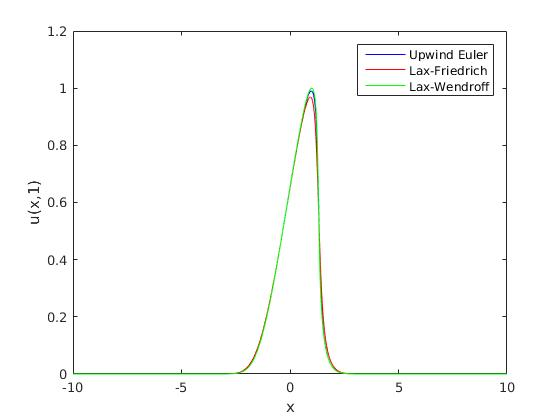
\includegraphics[width=\textwidth]{Images/8_ull_1.jpg}
  \caption{$t=1$}
\end{subfigure}
\begin{subfigure}[b]{0.45\textwidth}
  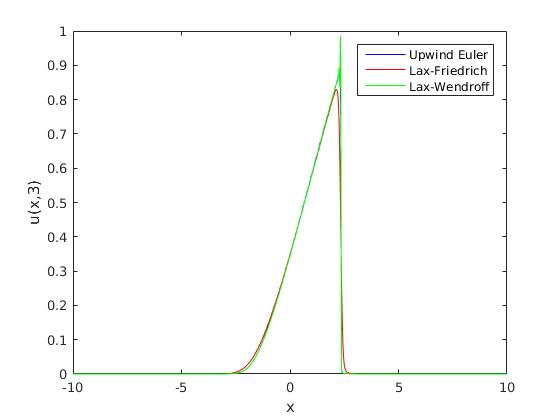
\includegraphics[width=\textwidth]{Images/8_ull_2.jpg}
  \caption{$t=3$}
\end{subfigure}
\begin{subfigure}[b]{0.45\textwidth}
  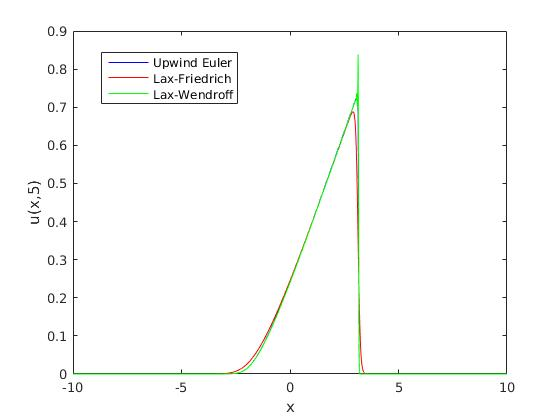
\includegraphics[width=\textwidth]{Images/8_ull_3.jpg}
  \caption{$t=5$}
\end{subfigure}
\begin{subfigure}[b]{0.45\textwidth}
  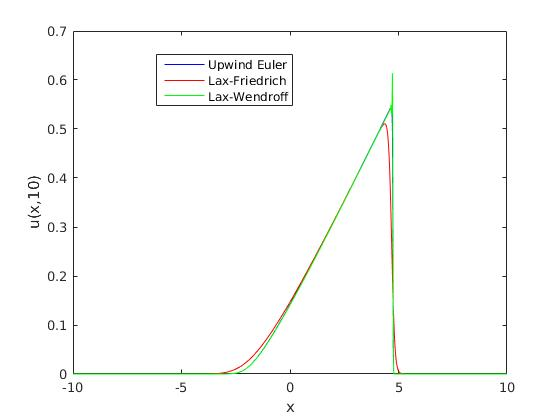
\includegraphics[width=\textwidth]{Images/8_ull_4.jpg}
  \caption{$t=10$}
\end{subfigure}
\caption{Evolution of Burgers' Equation using Upwind Euler, Lax-Friedrich and Lax-Wendroff}
\label{fig:burger_ull}
\end{figure}
%----------------------------------------------------------------------
\begin{figure}[H]
\centering
\begin{subfigure}[b]{0.45\textwidth}
  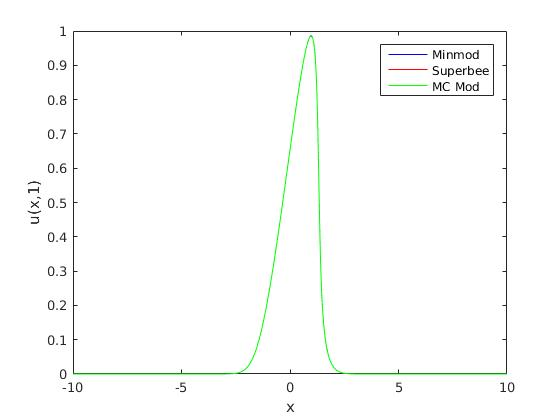
\includegraphics[width=\textwidth]{Images/8_msm_1.jpg}
  \caption{$t=1$}
\end{subfigure}
\begin{subfigure}[b]{0.45\textwidth}
  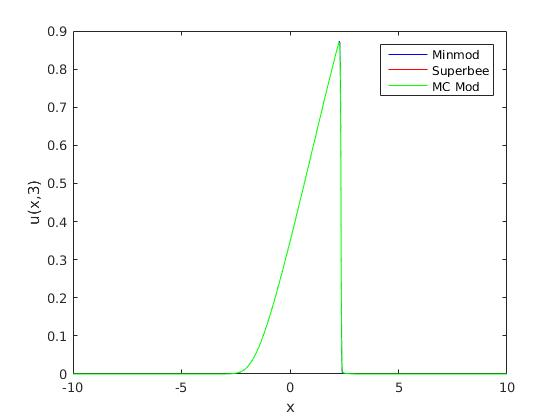
\includegraphics[width=\textwidth]{Images/8_msm_2.jpg}
  \caption{$t=3$}
\end{subfigure}
\begin{subfigure}[b]{0.45\textwidth}
  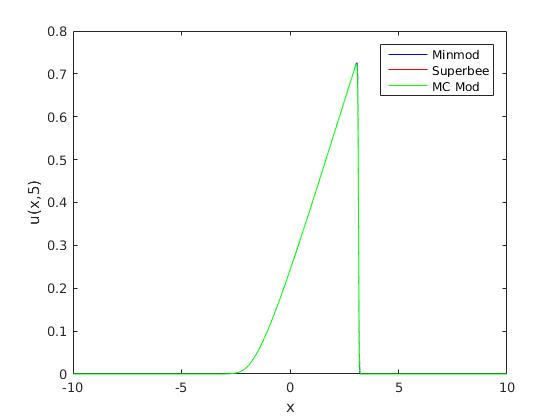
\includegraphics[width=\textwidth]{Images/8_msm_3.jpg}
  \caption{$t=5$}
\end{subfigure}
\begin{subfigure}[b]{0.45\textwidth}
  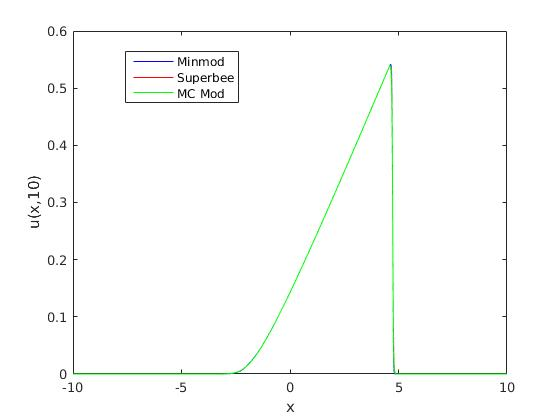
\includegraphics[width=\textwidth]{Images/8_msm_4.jpg}
  \caption{$t=10$}
\end{subfigure}
\caption{Evolution of Burgers' Equation using Minmod, Superbee and MC Mod}
\label{fig:burger_msm}
\end{figure}